% ATLAS uses a right-handed coordinate system, with origin located at the interaction point (IP). The $z$-axis runs along the beam line, the positive $x$-axis points towards the center of the LHC, and the positive $y$-axis points upwards. The positive $z$-axis is referred to as `side A', with the negative side referred to as `side C'.  More conveniently, polar coordinates are used in the transverse plane to take advantage of the cylindrical symmetry of the detector.
% The standard notation for polar coordinates is used:

% \begin{equation}
%     r = \sqrt{x^2 + y^2}
% \end{equation}\label{eq:transverse_radius}

% \begin{equation}
%     \varphi = \arctan\left(\frac{y}{x}\right)
% \end{equation}\label{eq:transverse_phi}

% \noindent{}The angle between the beam axis and the particles trajectory is defined as the polar angle $\theta$:

% \begin{equation}
%     \theta = \arctan\left(\frac{r}{z}\right)
% \end{equation}\label{eq:polar_angle}

% \noindent{}In particle physics it is more common to use the pseudorapidity $\eta$, which represents the angle of a particle with respect to the beam axis, and is defined as:

% \begin{equation}
%     \eta = -\ln\left(\tan\left(\frac{\theta}{2}\right)\right)
% \end{equation}\label{eq:pseudorapidity}

% \noindent{}Thus the commonly used, and preferred, coordinate system is represented by (r, $\varphi$, $\eta$) where the distance between two objects can be defined by:

% \begin{equation}
%     \Delta R = \sqrt{{(\Delta \eta)}^2 + {(\Delta \varphi)}^2}
% \end{equation}\label{eq:delta_R}

% \noindent{}An illustration of the coordinate system can be seen in Figure~\ref{fig:atlas_coordinate_system}.

% \begin{figure}
%     \centering
%     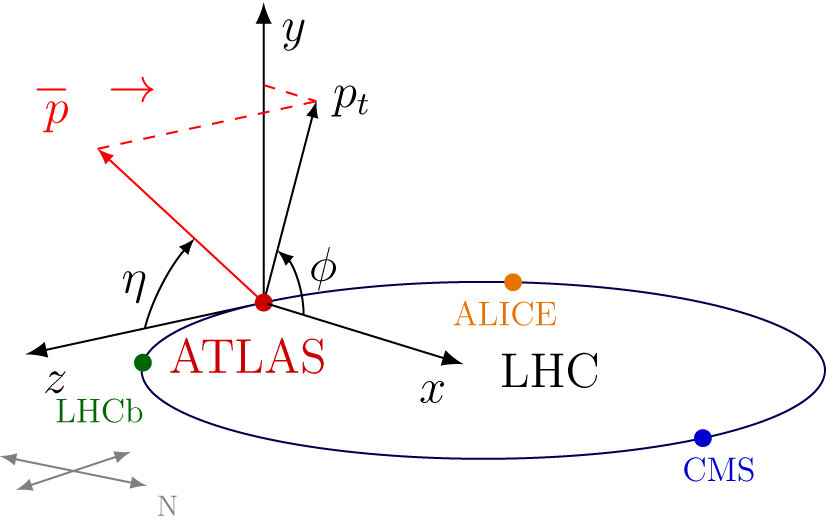
\includegraphics[width=0.9\textwidth]{figures/atlas/atlas_coordinate_system.jpg}
%     \caption{Depicted is the traditional (x,y,z) coordinate system overlaid with the cylindrical coordinate system used by physicists. Taken from~\cite{atlas_coordinate_system}}\label{fig:atlas_coordinate_system}
% \end{figure}

%%%%%%%%%%%%%%% revision
ATLAS uses a right-handed coordinate system with the origin at the interaction point (IP). The $z$-axis follows the beam line, positive $x$ points towards the LHC center, and positive $y$ upwards. The positive $z$ direction is referred to as `side A', and the negative `side C'.  Due to the detector's cylindrical symmetry, transverse polar coordinates are used where $r = \sqrt{x^2 + y^2}$ and $\varphi = \arctan\left(\frac{y}{x}\right)$. 
The angle between the beam axis and the particle's trajectory is defined as the polar angle $\theta = \arctan\left(\frac{r}{z}\right)$. In particle physics, pseudorapidity $\eta$ is preferred and is related to the polar angle via $\eta = -\ln\left(\tan\left(\frac{\theta}{2}\right)\right)$. The commonly used coordinate system is represented by (r, $\varphi$, $\eta$), where the distance between two objects can be defined as $\Delta R = \sqrt{{(\Delta \eta)}^2 + {(\Delta \varphi)}^2}$. An illustration of the coordinate system can be seen in Figure~\ref{fig:atlas_coordinate_system}.
\begin{figure}
    \centering
    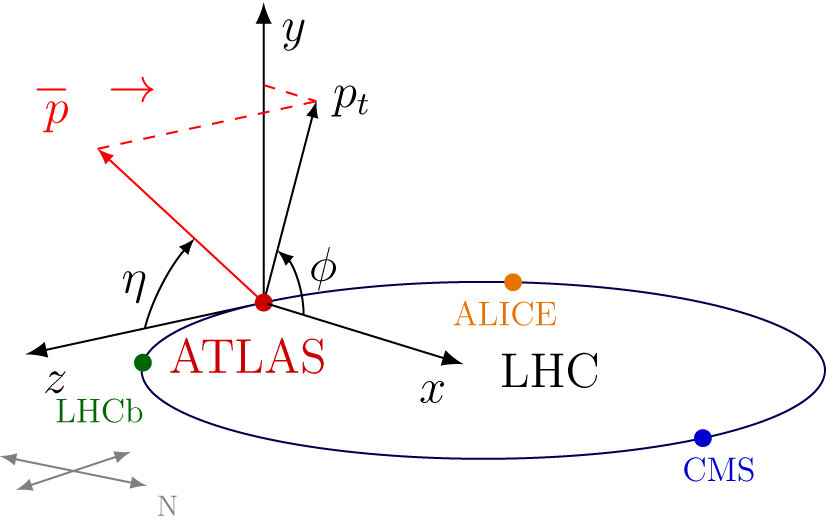
\includegraphics[width=0.9\textwidth]{figures/atlas/atlas_coordinate_system.jpg}
    \caption{Depicted is the traditional (x,y,z) coordinate system overlaid with the cylindrical coordinate system used by physicists. Taken from~\cite{atlas_coordinate_system}}\label{fig:atlas_coordinate_system}
\end{figure}